\documentclass{standalone}
\usepackage{amsmath,amssymb}
%matrix
\newcommand{\mt}[1]{\ensuremath{\mathbf{#1}}}
%vector
\newcommand{\vc}[1]{\ensuremath{\boldsymbol{#1}}}
%set
\newcommand{\st}[1]{\ensuremath{\mathcal{#1}}}
%time index
\newcommand{\tm}[1]{\ensuremath{\sp{(#1)}}}


%x
\newcommand{\x}[0]{\ensuremath{\vc{x}}}
%s
\newcommand{\s}[0]{\ensuremath{\vc{s}}}
%W
\newcommand{\W}[0]{\ensuremath{\mt{W}}}



\usepackage{pgf}
\usepackage{tikz}
\usetikzlibrary{arrows,automata,matrix}
\usepackage[latin1]{inputenc}
\begin{document}
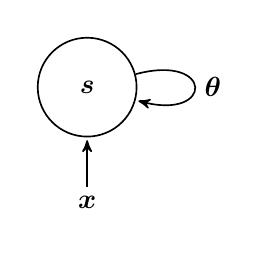
\begin{tikzpicture}[->,>=stealth',shorten >=1pt,auto,node distance=2.8cm,
                    semithick]
  \tikzstyle{every state}=[
  minimum size={10pt+width("$x^{(t-1)}$")}]
      \matrix (m) [matrix of nodes
      ,row sep=.25in,column sep=.25in] {
      \node[state](s) {$\vc{s}$}; \\
      \node[     ](x) {$\vc{x}$}; \\
      };
    

  \path (x) edge              node {} (s)
        (s) edge [loop right] node {$\vc{\theta}$} (s);
 
\end{tikzpicture}

\end{document}